
\documentclass[oneside,final]{beamer}

\usetheme{Berlin}

\usepackage[utf8]{inputenc}
\usepackage[T1]{fontenc}

\usepackage{pgf,pgfarrows,pgfnodes}

\usepackage{soul}
\usepackage{geometry}
\geometry{paper=a4paper,hmargin=1cm,vmargin=1cm}

\setbeamercolor{myhead}{fg=black,bg=white!90!blue}

\setbeamercolor{block1up}{fg=black,bg=white!60!green}
\setbeamercolor{block1down}{fg=black,bg=white!90!green}

\setbeamercolor{block2up}{fg=black,bg=white!60!red}
\setbeamercolor{block2down}{fg=black,bg=white!90!red}

\setbeamercolor{block3up}{fg=black,bg=white!60!blue}
\setbeamercolor{block3down}{fg=black,bg=white!90!blue}

\setbeamercolor{example1up}{fg=black,bg=white!90!black}
\setbeamercolor{example1down}{fg=black,bg=white}

\usepackage{graphicx}

\usepackage[absolute,overlay]{textpos}
\setlength{\TPHorizModule}{1cm}
\setlength{\TPVertModule}{1cm}
\textblockorigin{0cm}{0cm}

% utopia font set.
\usepackage[expert,widespace]{fourier}
\usepackage[scaled=0.875]{helvet}
\renewcommand{\ttdefault}{lmtt}

\pagestyle{empty}

\newenvironment{pgfdrawing}{
\begin{textblock}{1}(0,29)
\begin{pgfpicture}{0cm}{0cm}{1cm}{1cm}
\begin{pgfscope}}{
\end{pgfscope}
\end{pgfpicture}
\end{textblock}
}

\newcommand\showgrid{
\begin{pgfdrawing}
    \color{red}
    \pgfsetlinewidth{0.2pt}
    \pgfgrid[step={\pgfpoint{1cm}{1cm}}]{\pgfxy(0,0)}{\pgfxy(21,30)}
    \pgfsetlinewidth{1pt}
    \pgfgrid[step={\pgfpoint{5cm}{5cm}}]{\pgfxy(0,0)}{\pgfxy(21,30)}
    \pgfputat{\pgfxy(0.2,0.2)}{\pgfbox[left,bottom]{0,0}}
    \pgfputat{\pgfxy(0,0)}{\pgfcircle[fill]{\pgfxy(0,0)}{0.1cm}}
\end{pgfdrawing}
}

\newcommand\drawarrow[1]{
\begin{pgfdrawing}
\color{black}
\pgfsetlinewidth{2pt}
\pgfsetendarrow{\pgfarrowtriangle{7pt}}
\pgfsetstartarrow{\pgfarrowcircle{2pt}}
#1
\end{pgfdrawing}
}


\begin{document}

% enable grid mode
% \showgrid

% title
\begin{textblock*}{19cm}(1cm,1cm)
\noindent%
\begin{beamerboxesrounded}[shadow=false,upper=myhead,lower=myhead]{}
\centering \scalebox{1.5}{\Huge \textrm{\so{POSTER TITLE}}} \\[.5cm]
\Large Marek Kubiak \hspace{2cm} Przemysław Wesołek \\[.3cm]
\large Poznań University of Technology, ul.~Piotrowo 2, Poland
\end{beamerboxesrounded}
\end{textblock*}

% arrows
\drawarrow{\color{red}\pgfxycurve(6.2,5)(8,5)(8,3)(9.5,3)}
\drawarrow{\color{red}\pgfxycurve(5.5,11)(-5,12)(1.5,5)(3.5,5)}

% content blocks
\begin{textblock*}{9cm}(1cm,5cm)\noindent%
\begin{beamerboxesrounded}[shadow=false,upper=block1up,lower=block1down]{\large\textbf{Theory}}
Lorem ipsum dolor sit amet, consectetuer adipiscing elit. Aenean lacus dui, lacinia et, placerat vitae, lobortis in, lorem. Curabitur porttitor urna et neque congue dignissim. Nunc adipiscing sapien iaculis urna. Nullam lorem massa, faucibus eu, venenatis pretium, laoreet vel, nulla. Donec pede lectus, lacinia ac, volutpat sit amet, ultricies sed, lacus. Nunc nibh nulla, pellentesque quis, luctus id, lobortis eget, metus. Integer hendrerit lorem ultrices dui. Quisque tristique. Integer pulvinar. In hac habitasse platea dictumst. Maecenas volutpat, lectus sed pulvinar ullamcorper, augue tortor sollicitudin orci, ut ultricies ligula elit non libero. Etiam bibendum nibh eget augue lacinia dictum. Nunc erat. Sed libero purus, volutpat ut, vestibulum vitae, scelerisque eu, justo. Etiam sed eros et erat ornare pretium. Quisque varius. Donec lacinia lorem in nunc. Nulla facilisi. Integer egestas tortor dictum nulla. Vestibulum semper urna vel enim.
\par\medskip Quisque commodo gravida orci. Phasellus adipiscing mattis nunc. Quisque et leo. Nullam vel pede. Sed id erat. In hac habitasse platea dictumst. Duis ut velit at lacus consectetuer interdum. Nulla orci erat, fermentum quis, tincidunt nec, posuere sed, dui. Donec nec turpis sit amet ligula scelerisque venenatis. Aenean a leo. Quisque euismod. Suspendisse accumsan bibendum metus. Donec pede. Vestibulum pellentesque semper tortor. Curabitur semper ligula sed massa.
\end{beamerboxesrounded}
\end{textblock*}

\begin{textblock*}{8cm}(1cm,18cm)\noindent%
\begin{beamerboxesrounded}[shadow=false,upper=block1up,lower=example1down]{\large\textbf{Example}}
\centering 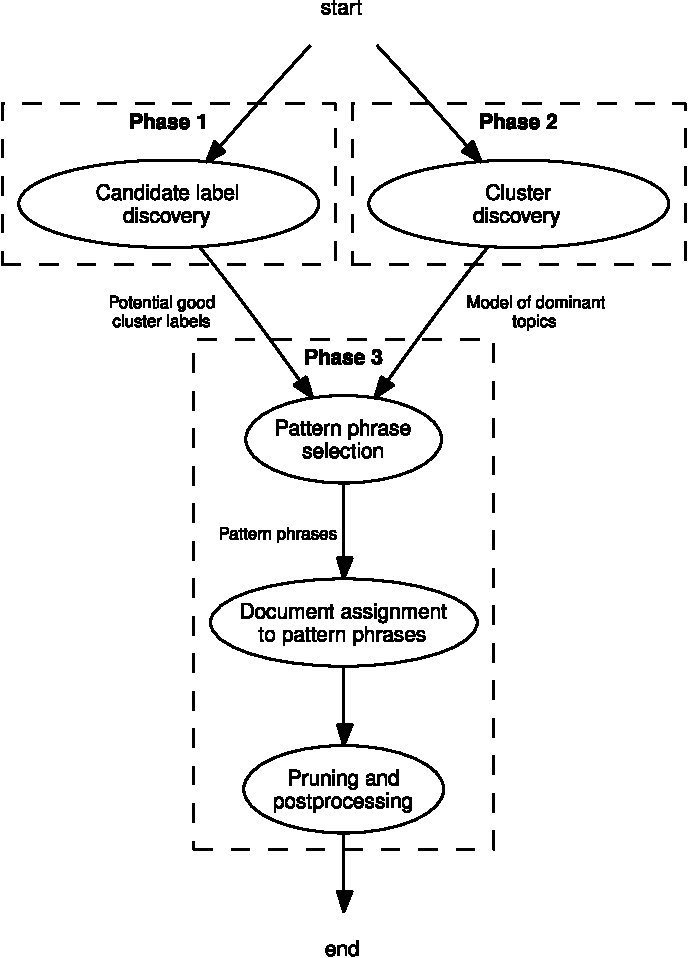
\includegraphics[width=.7\linewidth]{dcf-phases} \par
\end{beamerboxesrounded}
\end{textblock*}

\begin{textblock*}{9cm}(11cm,5cm)\noindent%
\begin{beamerboxesrounded}[shadow=false,upper=block2up,lower=block2down]{\large\textbf{Experiments}}
Lorem ipsum dolor sit amet, consectetuer adipiscing elit. Aenean lacus dui, lacinia et, placerat vitae, lobortis in, lorem. Curabitur porttitor urna et neque congue dignissim. Nunc adipiscing sapien iaculis urna. Nullam lorem massa, faucibus eu, venenatis pretium, laoreet vel, nulla. Donec pede lectus, lacinia ac, volutpat sit amet, ultricies sed, lacus. Nunc nibh nulla, pellentesque quis, luctus id, lobortis eget, metus. Integer hendrerit lorem ultrices dui. Quisque tristique. Integer pulvinar. In hac habitasse platea dictumst. Maecenas volutpat, lectus sed pulvinar ullamcorper, augue tortor sollicitudin orci, ut ultricies ligula elit non libero. Etiam bibendum nibh eget augue lacinia dictum. Nunc erat. Sed libero purus, volutpat ut, vestibulum vitae, scelerisque eu, justo. Etiam sed eros et erat ornare pretium. Quisque varius. Donec lacinia lorem in nunc. Nulla facilisi. Integer egestas tortor dictum nulla. Vestibulum semper urna vel enim.
\par\medskip Quisque commodo gravida orci. Phasellus adipiscing mattis nunc. Quisque et leo. Nullam vel pede. Sed id erat. In hac habitasse platea dictumst. Duis ut velit at lacus consectetuer interdum. Nulla orci erat, fermentum quis, tincidunt nec, posuere sed, dui. Donec nec turpis sit amet ligula scelerisque venenatis. Aenean a leo. Quisque euismod. Suspendisse accumsan bibendum metus. Donec pede. Vestibulum pellentesque semper tortor. Curabitur semper ligula sed massa. Proin in diam ac mauris venenatis dapibus. Sed vulputate libero et nulla. Nam ullamcorper pharetra mi.
\end{beamerboxesrounded}
\end{textblock*}

\begin{textblock*}{10cm}(10cm,20cm)\noindent%
\begin{beamerboxesrounded}[shadow=false,upper=block3up,lower=block3down]{\large\textbf{Results}}
Lorem ipsum dolor sit amet, consectetuer adipiscing elit. Aenean lacus dui, lacinia et, placerat vitae,
\begin{equation*}
2 + 2 = 4
\end{equation*}
lobortis in, lorem. Curabitur porttitor urna et neque congue dignissim. Nunc adipiscing sapien iaculis urna. Nullam lorem massa, faucibus eu, venenatis pretium, laoreet vel, nulla. Donec pede lectus, lacinia ac, volutpat sit amet, ultricies sed, lacus. Nunc nibh nulla, pellentesque quis, luctus id, lobortis eget, metus. Integer hendrerit lorem ultrices dui. Quisque tristique. Integer pulvinar. In hac habitasse platea dictumst. Maecenas volutpat, lectus sed pulvinar ullamcorper, augue tortor sollicitudin orci, ut ultricies ligula elit non libero. Etiam bibendum nibh eget augue lacinia dictum. Nunc erat. Sed libero purus, volutpat ut, vestibulum vitae, scelerisque eu, justo. Etiam sed eros et erat ornare pretium. Quisque varius. Donec lacinia lorem in nunc. Nulla facilisi. Integer egestas tortor dictum nulla. Vestibulum semper urna vel enim.
\end{beamerboxesrounded}
\end{textblock*}

% background last
\begin{textblock*}{0cm}(0cm,0cm)
\noindent%

\includegraphics[angle=90,width=\paperwidth,height=\paperheight]{background}
\end{textblock*}

\end{document}
